\documentclass[pdf]{beamer}
\usepackage[slovak]{babel}
\usepackage[utf8]{inputenc}
\usepackage{hyperref}
\usepackage{breakurl} 
\usepackage{listings}

\lstdefinelanguage{JavaScript}{
  keywords={typeof, new, true, false, catch, function, return, null, catch, switch, var, if, in, while, do, else, case, break, then, yield, const, ajax},
  basicstyle=\small,
  keywordstyle=\color{blue}\bfseries,
  ndkeywords={class, export, boolean, throw, implements, import, this},
  ndkeywordstyle=\color{darkgray}\bfseries,
  identifierstyle=\color{black},
  sensitive=false,
  comment=[l]{//},
  morecomment=[s]{/*}{*/},
  commentstyle=\color{purple}\ttfamily,
  stringstyle=\color{red}\ttfamily,
  morestring=[b]',
  morestring=[b]",
  frame=lines,
  numbers=left,
  basicstyle=\scriptsize,
  numberstyle=\scriptsize,
  stepnumber=1,
  numbersep=8pt,
  showstringspaces=false,
  captionpos=b
}
\renewcommand{\lstlistingname}{Code sample}


\title{Obecné konfiguračné rozhranie pre virtuálne stroje}
\subtitle{Bakalárska práca}
\author{Martin Krajňák}
\date{2017}

\usetheme{Warsaw}

\begin{document}

\begin{frame}
\titlepage
\end{frame}


\begin{frame}
\frametitle{Motivácia súčasný stav - oVirt WebAdmin}
\begin{itemize}
\item súčasná implementácia je:
\begin{itemize}
\item pomalá
\item náchylná na chyby, problémso stavom dialógu
\item s pribudajúcim kódom vzniká viac chýb (callback hell)
\end{itemize}
\item technológia GWT už nie je v aktívnom vývoji (Google)
\item virtuálny stroj 
\begin{itemize}
\item veľký počet závislostí, ktoré su vzájomne ovplyvniteľné
\item chýbajúca dokumentácia závislostí
\end{itemize}
\end{itemize}
\end{frame}


\begin{frame}
\frametitle{Ciele práce - projekt oVirt WebUI}
\begin{block}{Backend}

\begin{itemize}
\item dva nezávyslé moduly:

\begin{itemize}
\item oVirt REST API
\item ManageIQ REST API
\end{itemize}

\item jQuery, Ajax
\end{itemize}

\end{block}

\begin{block}{Redux-saga middleware}
\begin{itemize}
\item Redux-saga:
\begin{itemize}
\item riadenie asynchrónnych operácii
\item riešenie závislostí virtuálneho stroja
\item konverzia entít na vnútornú reprezentáciu
\item odosielanie požiadavkov a vyhodnotenie odpovede
\end{itemize}
\item Redux - načítanie a uloženie dát potrebných pre prácu s dialógmi (virtuálne stroje, clustre, šablony)
\end{itemize}
\end{block}

\end{frame}


\begin{frame}

\begin{block}{Frontend - ReactJS}
\begin{itemize}
\item návrh bezstavových komponent s dôrazom na znovupoužiteľnosť
\item návrh hlavných komponent - dialógov
\item použitie štýlov z knižnice Patternfly
\item Redux 

\begin{itemize}
\item správa stavu aplikácie/dialógov
\item prepojenie na middleware
\item zachovanie konzistencie a predvídateľnosti stavu
\end{itemize}

\item JSX 
\end{itemize}
\end{block}

\end{frame}

\begin{frame}
\frametitle{Realizácia}

\begin{figure}[h]
\center{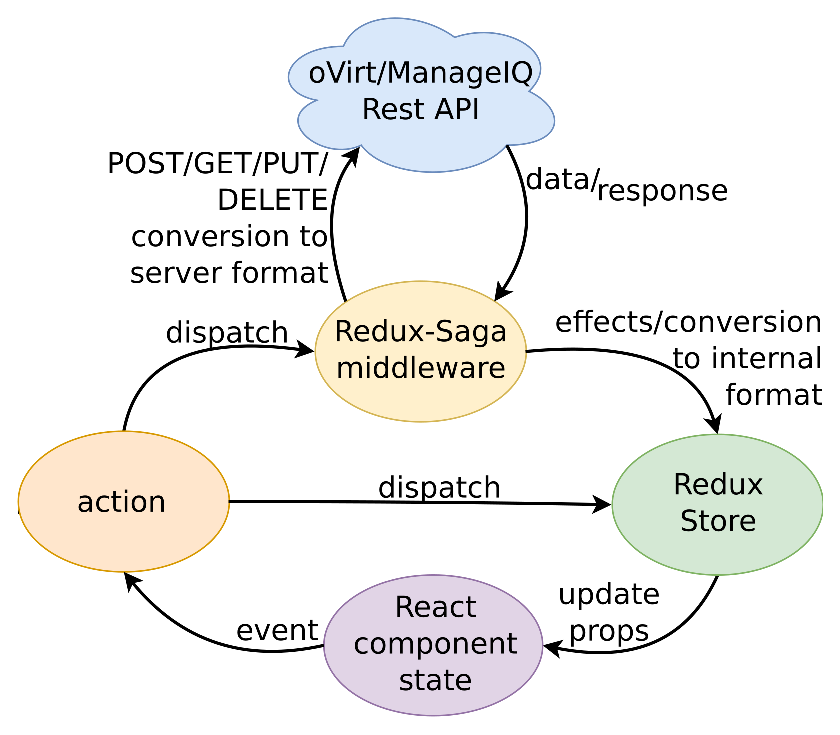
\includegraphics[scale=0.6]{application_architecture.eps}}
\label{labelledSelect}
\end{figure} 

\end{frame}

\begin{frame}
\frametitle{oVirt REST API vs ManageIQ REST  API}

\begin{block}{oVirt REST API} 
podpora takmer všetkých vlastností a akcií
\end{block}

\begin{block}{ManageIQ - problémy pri implementácii} 
\begin{itemize}
\item nefunkčná CORS implementácia:

\begin{enumerate}
\item nahlásenie problému
\item aplikovanie a testovanie navrhnutých opráv
\item problém vyriešený len čiastočne - entity najvyššej úrovne
\item dočasné riešenie - absolútne vypnutie bezpečnosti prehliadača
\end{enumerate}

\item nedostatočné/žiadne pokrytie entít
\begin{enumerate}
\item chýbajúce informácie a akcie
\item neschopnosť určenia základných vzťahov (šablona, cluster)
\end{enumerate}

\item zlé rozloženie virtuálnych strojov - spomaľovanie

\end{itemize}
\end{block}

\end{frame}

\begin{frame}
\frametitle{Realizácia}

\begin{figure}[h]
\center{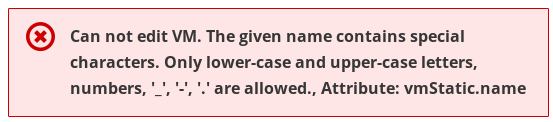
\includegraphics[width=6cm]{alert.png}}
\label{labelledSelect}
\end{figure}

\begin{figure}[h]
\center{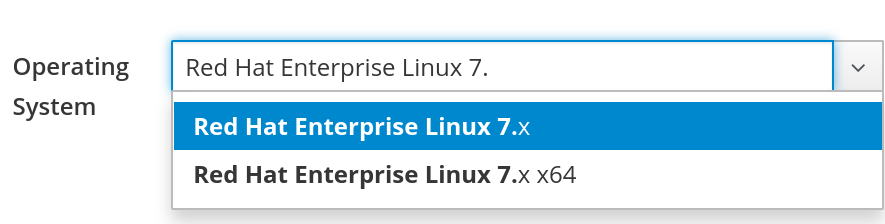
\includegraphics[width=6cm]{LabeledSelect.png}}
\label{labelledSelect}
\end{figure} 

\begin{figure}[h]
\center{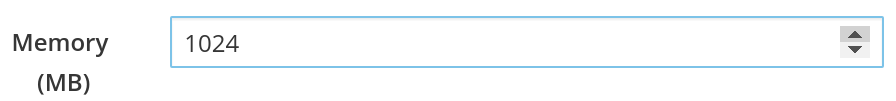
\includegraphics[width=6cm]{LabelledTextField-number.png}}
\label{labelledSelect}
\end{figure} 


\begin{figure}[h]
\center{
\includegraphics[width=2cm]{LabeledSwitch.png}}
\label{labelledSelect}
\end{figure}

\end{frame}


\end{document}